\section{Polynomdivision}\index{Polynomdivision}
Die Polynomdivision wird eingesetzt um entweder den Grad eines Polynoms zu verringern oder die Bruchform einer gebrochenrationalen Funktion in die Summenform umzuwandeln. 
\subsection{Polynomdivision bei Polynomen}\index{Polynomdivision!Polynome}\label{polynomdivision}

    Bei einem Polynom wird die Polynomdivision angewendet um den Grad des Polynoms zu verringern und die Faktorisierte Darstellung des Polynoms zu erzeugen. Als Beispiel wird hier die Funktion $f(x) = x^3-6x^2-x+6$ verwendet. Hierbei ist es Ziel, dass man das Polynom als Produkt der Nullstellen darstellen kann.\\
    Es gilt folgender Zusammenhang: $$f(x) = x^3-6x^2-x+6 =  \polyfactorize{x^3-6x^2-x+6}.$$ Aus dieser Darstellung folgt, dass die Funktion $f$ die Nullstellen $x_1 = -1, x_2 = 1$ und $x_3= 6$ hat. Um die Polynomdivision durchführen zu können, muss man als erstes eine Nullstelle kennen und dann das Polynom durch diese Nullstelle teilen. Nach der Division erhält man jeweils eine neues Polynom geringeren Grades. Dieses Polynom muss dann wieder mit der Polynomdivision vom Grad reduziert werden.
    \begin{bsp}{Die Polynomdivision bei Polynomen}{} 
Man rät die Nullstelle $x=1$ und führt jetzt die Polynomdivision durch:\\
 \polylongdiv{x^3- 6x^2 - x +6}{x-1}\\
 Das neue Polynom kann jetzt mit der Mitternachtsformel weiter bearbeitet werden oder erneut durch eine Polynomdivision bearbeitet werden. \\
  \polylongdiv{x^2-5x^1 -6}{x+1}\\
  oder
  $$ x_{1,2} = \dfrac{5\pm \sqrt{(-5)^2 - 4\cdot 1 \cdot (-6)}}{2\cdot 1} = \dfrac{5 \pm \sqrt{49} }{2} = \dfrac{5\pm 7}{2}$$
 $$ x_1 = -1$$
 $$ x_2= 6$$
\begin{center}
    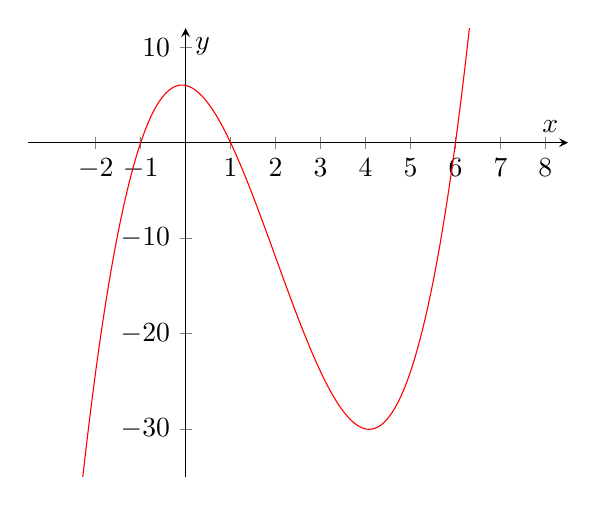
\begin{tikzpicture}
        \begin{axis}[xmin= -3.5, xmax = 8.5, ymin= -35, ymax= 12,
        axis lines = middle, 
        xtick={-2, -1, 0, ..., 8},
        xlabel = $x$,
        ylabel=$y$]
            \addplot[color= red, samples = 300, domain= -2.5:6.5]{x^3-6*x^2-x+6};
        \end{axis}
    \end{tikzpicture}     
\end{center}
\end{bsp}
\begin{b8d}{Rest der Polynomdivision}{rest}
  Bei der Polynomdivision zur Bestimmung der Nullstellen eines Polynoms treten \textcolor{red}{keine Restterme} auf.   
\end{b8d}
\subsection{Polynomdivision bei gebrochenrationalen Funktionen}\index{Polynomdivision!gebrochenrationale Funktionen}\label{polynomdivisionBruch}
Die zweite Anwendung der Polynomdivision besteht in der Umwandlung der Bruchform in die Summenform der ganzrationalen Funktionen. Hierbei wird die Polynomdivision durchgeführt indem man den Zähler der Funktion durch seinen Nenner dividiert.
\begin{bsp}{Polynomdivision ganzrationaler Funktionen}{}
Gegeben ist die Funktion $$f(x)=\dfrac{x^2+x-2}{2x-4}$$ mit $\mathds{D}_f=\mathds{R}\setminus \left\{ 2 \right\}$. Durch die Polynomdivision soll die Bruchform in die Summenform überführt werden.\\
\polylongdiv{x^2+x-2}{2x-4}\\
Damit lautet die Summenform wie folgt:
$$f(x)=\dfrac{x^2+x-2}{2x-4} = \dfrac{1}{2} x +\dfrac{3}{2} +\dfrac{4}{2x-4} $$
\end{bsp}
\section{Symmetrie} \index{Symmetrie}
Die Untersuchung der Symmetrie erfolgt für Funktionen immer nach dem selben Muster. Es wird im allgemeinen Untersucht, ob entweder \begin{equation}\label{f(x)}
    f(-x) = f(x)
\end{equation} oder 
\begin{equation} \label{-f(x)}
f(-x) = -f(x) 
\end{equation} gilt. Für die Gleichung \ref{f(x)} ist der Graph der Funktion $f$ achsensymmetrisch zur y-Achse. Für die Gleichung \ref{-f(x)} ist der Graph der Funktion $f$ punktsymmetrisch zum Ursprung. Gilt keine der beiden Gleichungen kann keine Aussage zur Symmetrie zur y-Achse bzw. zum Ursprung getroffen werden. 
\begin{center}
    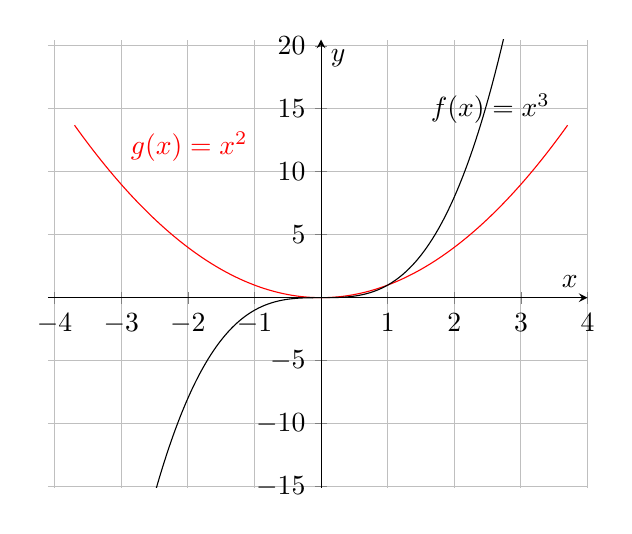
\begin{tikzpicture}
        \begin{axis}[xmin= -4.1, xmax = 4, ymin= -15.1, ymax= 20.5,
        axis lines = middle, 
        ymajorgrids=true,
        xmajorgrids=true,
        xtick={-4, -3,  ..., 2, 3, 4},
        ytick={-15, -10, -5, ..., 20},
        xlabel = $x$,
        ylabel=$y$]
            \addplot[color = red, samples = 300, domain= -3.7:3.7]{x^2};
         \draw (1.5,15)   node [right] {$f(x) = x^3$};  
            \addplot[color= black, samples = 300, domain= -3.7:3.7]{x^3};
            \draw (-3,12)   node [right] {\textcolor{red}{$g(x) = x^2$}}; 
            
        \end{axis}
    \end{tikzpicture}  
\end{center}
\section{Übersicht von Ableitungsregeln mit Beispielen} \index{Ableitung! Übersicht}
\subsection{Allgemeine Ableitungsregeln}\index{Ableitungsregeln! Allgemeine Ableitungsregln}
\begin{merke}{Allgemeine Ableitungsregeln}{}
\begin{multicols}{2}
\begin{itemize}
    \item Ableitung einer Konstanten:
    \begin{gather*} 
	f(x) = c \hspace{0.2cm}\text{mit} \hspace{0.2cm} c \in \mathds{R}\\ 
	f'(x) = 0
	\end{gather*}
    \item Ableitung der Ursprungsgeraden:
    \begin{gather*} 
	f(x) = x \\ 
	f'(x) = 1
	\end{gather*} 
     \item Ableitung einer allgemeinen Geraden:
    \begin{gather*} 
	f(x) = m\cdot x + t  \hspace{0.2cm}\text{mit} \hspace{0.2cm} m,t \in \mathds{R}\\ 
	f'(x) = m
	\end{gather*}
 \item Ableitung einer allgemeinen Potenzfunktion:
    \begin{gather*} 
	f(x) = x^n  \hspace{0.2cm}\text{mit} \hspace{0.2cm} n \in \mathds{N}\\ 
	f'(x) =n \cdot x^{n-1}
	\end{gather*}
\end{itemize}    
\end{multicols}
\end{merke}
\subsection{Ableitungsregeln von Funktionen}\index{Ableitungsregeln! Funktionen}
\begin{defi}{Ableitungsfunktionen}{}\phantomsection\label{AbleitungEFunktion}
\begin{multicols}{2}
\begin{itemize}
    \item Ableitung der Summe von Funktionen:
    \begin{gather*} 
	f(x) = u(x) + v(x) \\
	f'(x) = u'(x)+ v'(x)
	\end{gather*}
     \item Ableitung einer Funktion mit Vorfaktor:
    \begin{gather*} 
	f(x) = a\cdot u(x)  \\
	f'(x) = a\cdot u'(x) 
	\end{gather*}
       \item Ableitung des Produktes von zwei Funktionen:
    \begin{gather*} 
	f(x) = u(x) \cdot v(x)  \\
	f'(x) = u'(x) \cdot v(x) + u(x) \cdot v'(x)
	\end{gather*}     
        \item Ableitung des Quotienten von zwei Funktionen:
    \begin{gather*} 
	f(x) = \dfrac{u(x)}{v(x)}  \\
	f'(x) = \dfrac{u'(x)\cdot v(x) - u(x) \cdot v'(x)}{(v(x)^2)}
	\end{gather*} 
         \item Ableitung einer verketteten Funktion:

   \begin{gather*} 
	f(x) = u(v(x))  \\
	f'(x) = u'(v(x)) \cdot v'(x)
	\end{gather*} 

\end{itemize}   
\end{multicols}
\end{defi}
\subsection{Ableitung von Grundfunktionen}\index{Ableitungsregeln! Grundfunktionen}
\begin{merke}{Ableitungen von Grundfunktionen}{}
\begin{itemize}
 \item Trigonometrische Funktionen:
    \begin{gather*} 
	f(x) = \sin({x})  \\
	f'(x) = \cos({x})\\
 g(x) = \cos{(x)}\\
 g'(x) = -\sin{(x)}	\end{gather*}
\item e-Funktion
\begin{gather*} 
	f(x) = e^x  \\
	f'(x) = e^x
	\end{gather*}
 \item Logarithmusfunktion
 \begin{gather*} 
	f(x) = \ln{(x)}   \hspace{0.2cm} \text{mit} \hspace{0.2cm} x\in \mathds{R}\setminus \{0\}\\
	f'(x) = \dfrac{1}{x}
	\end{gather*}
 \item Quadratwurzel
 \begin{gather*} 
	f(x) = \sqrt{x} = x^{\frac{1}{2}}   \hspace{0.2cm} \text{mit} \hspace{0.2cm} x\in \mathds{R}\setminus \{0\} \\
 f'(x) = \dfrac{1}{2} \cdot x^{-\frac{1}{2} }= \dfrac{1}{2\cdot \sqrt{x}} 
 \end{gather*}
  \item allgemeine Wurzel
 \begin{gather*} 
	f(x) = \sqrt[n]{x} = x^{\frac{1}{n}}   \hspace{0.2cm} \text{mit} \hspace{0.2cm} x\in \mathds{R}\setminus \{0\}  \hspace{0.2cm} \text{und} \hspace{0.2cm} n\in \mathds{N} \\
 f'(x) = \dfrac{1}{n} \cdot x^{ \frac{1}{n} - 1}= \dfrac{1}{n\cdot \sqrt[n-1]{x}} 
 \end{gather*}
\end{itemize}
\end{merke}
\subsection{Beispiele der Ableitungsregeln}\index{Ableitungsregeln! Beispiele}\label{Ableitungen}
\begin{bsp}{Beispiele für die Ableitungsregln}{}
\begin{enumerate}
    \item $f(x) = 5 \longrightarrow f'(x) = 0$
    \item $f(x) = -3x +7 \longrightarrow f'(x) = -3 $
    \item $f(x) = x^6 \longrightarrow f'(x) = 6\cdot x^5$
    \item $f(x) = -2x^4+2x-1 \longrightarrow f'(x) = -2\cdot 4\cdot x^3 + 2 = -8\cdot x^3 +2$
    \item $f(x) = e^x \cdot (4x^3 -3) \longrightarrow f(x) = e^x \cdot (4x^3-3) + e^x \cdot (12x^2)$
    \item $f(x) = \dfrac{-x^4+ 2x^3 + 5 }{(2x-1)} \longrightarrow f'(x) = \dfrac{(2x-1)\cdot (-4x^3+6x^2) - (-x^4 +2x^3 + 5)\cdot 2 }{(2x-1)^2}$ \\[0.2cm]
    Als Eselsbrücke kann man sich folgenden Zusammenhang merken: \\[0.2cm]
    $f(x) = \dfrac{N}{Z} \longrightarrow f'(x) = \dfrac{{N}{\cdot {AZ} -{}Z}\cdot {AN}}{{N}^2}$ oder\\[0.2cm]  {\bfseries\color{red}N}enner mal {\bfseries\color{red}A}bleitung {\bfseries\color{red}Z}ähler - {\bfseries\color{red}Z}ähler mal {\bfseries\color{red}A}bleitung {\bfseries\color{red}N}enner geteilt durch {\bfseries\color{red}N}enner im Quadrat
    \item $f(x)= e^{2x^5-x^3+2 }\longrightarrow f'(x) = e^{2x^5-x^3 + 2} \cdot (10x^4 -3x^2)$
\end{enumerate}
\end{bsp}
\section{Elementare gebrochen-rationale Funktionen} \index{Funktionen!Gebrochen-rationale Funktionen!allgemeine Betrachtungen}
\subsection{Allgemeine Betrachtungen}
\label{elemgebrat}In der Jahrgangsstufe 8 wurden bereits einfache gebrochen-rationale Funktionen betrachtet. Diese Funktionen gehorchten dem Term der Form $$f: x\longrightarrow \dfrac{a}{x+b} +c$$ mit $a \in \mathds{R}\setminus\{0\}$ und $b,c\in\mathds{R}$. Hierbei wird durch die Untersuchung von Graphen klar, dass die Parameter $b,c$ eine Verschiebung des Graphen der Funktion $g$ mit $g:x\longrightarrow \dfrac{a}{x}$ in x- bzw. in y-Richtung realisieren. Die Einführung der Parameter $b,c$ als Asymptoten des Graphen $G_f$ erfolgt daran anschließend. 
\begin{bsp}{Elementare gebrochen-rationale Funktionen}{}
Am Beispiel der Funktion $f(x) = \dfrac{-2}{x+4} - 2$ mit $\mathds{D}_f = \mathds{R}\setminus\{-4\}$ sollen beispielhaft diese Überlegungen durchgeführt werden. Die Definitionslücke ergibt sich aus der Nullstelle des Nennerpolynoms $n(x) = x+4$. 
 \begin{equation*}
    \begin{split}
        0 &= x+4 \hspace{0.5 cm} | -4\\
        x&=-4 
       \end{split}
\end{equation*}
Hierbei ergibt sich aus der Definitionslücke die senkrechte Asymptote. Die waagerechte Asymptote ergibt sich aus dem additiven Parameter $-2$ da die Funktionswerte sich beliebig genau diesem Wert annähern ihn aber nie annehmen. Allgemeinere Betrachtungen des Graphen sind durch die linearen Transformationen \ref{lintrans} erklärbar
\begin{center}
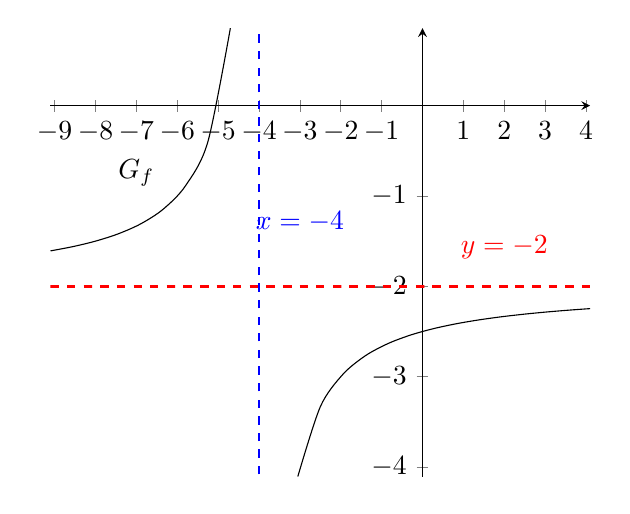
\begin{tikzpicture}
    \begin{axis}[domain=-9.1:4.1, restrict y to domain=-5:5, axis x line=center, axis y line=center,%
xtick={-9,...,4}, ytick={-5,...,5}]
        \addplot[mark=none  plot[samples=300,smooth]{-2/(x+4) -2};
        \addplot[line width=1pt,mark=none, color=red, dashed]  plot[samples=300,smooth]{-2-0*x};
        \draw [line width=1pt, color = blue, dashed] (-4,-5) -- (-4,5);
        \draw (-7,-1)   node [above] {$G_{f}$};
        \draw[red] (2,-1.8)   node [above] {$y=-2$};
        \draw[blue] (-3,-1.5)   node [above] {$x=-4$};
    \end{axis}
\end{tikzpicture}
\end{center}
\end{bsp}
\subsection{Grenzwertbetrachtungen bei gebrochen-rationalen Funktionen} \index{Funktionen!Gebrochen-rationale Funktionen!Grenzwertbetrachtungen} \label{Fallgebrochenrational}
Die Grenzwertbetrachtungen bei gebrochen-rationalen Funktionen kann über die Auswertung von Zähler- und Nennergrad erfolgen. Hierbei versteht man unter dem Grad eines Polynoms den höchsten vorkommenden Exponenten. Man unterscheidet dabei 4 mögliche Fälle.
\begin{merke}{Fallunterscheidungen}{}
Die Art der Asymptote einer gebrochen-rationalen Funktion $f(x)=\dfrac{Z(x)}{N(x)}$ mit $\mathds{D} = \mathds{D}_{\text{max}}$ hängt vom Grad der Polynome des Zähler als auch des Nenners ab.
\begin{enumerate}
    \item Grad des Zählerpolynoms $<$ Grad des Nennerpolynoms\\
    Durch Grenzwertbetrachtungen kann nachgewiesen werden, dass die x-Achse die waagerechte Asymptote ist. Daraus folgt $$\lim_{x\longrightarrow \infty} f(x) = \lim_{x\longrightarrow -\infty} f(x) = 0$$
\item  Grad des Zählerpolynoms $=$ Grad des Nennerpolynoms\\ Bei Grenzwertuntersuchungen findet man eine waagerechte Asymptote die parallel zur x-Achse verläuft. Hierbei ergibt sich die waagerechte Asymptote aus dem Quotienten der Vorfaktoren der größten Exponenten.\\ Als Beispiel wird die Funktion $f(x)= \dfrac{2x^2}{3x^2-x+1}$, hierbei folgt aus der Grenzwertbetrachtung: $$\lim_{x\longrightarrow \infty} f(x) = \lim_{x\longrightarrow \infty} \dfrac{2x^2}{3x^2-x+1} = \dfrac{2}{3}$$ und $$\lim_{x\longrightarrow -\infty} f(x) = \lim_{x\longrightarrow -\infty} \dfrac{2x^2}{3x^2-x+1} = \dfrac{2}{3}$$
\item Grad des Zählerpolynoms $>$ Grad des Nennerpolynoms\\
In diesem Fall existiert eine schräge Asymptote. Diese ist direkt aus der Summenform ablesbar. \\ Als Beispiel wird die Funktion $f(x)= \dfrac{x^2+1,5x}{2x-1} = \dfrac{1}{2}x+1+\dfrac{1}{2x-1}$ betrachtet. Die schräge Asymptote hat damit die Gleichung $y= \dfrac{1}{2}x+1$.
\item Grad des Zählerpolynoms $>$ Grad des Nennerpolynoms +1\\
Für diesen Fall ergibt sich eine Näherungskurve vom Grad $n\geq 2$. Die Funktion\\ $f(x) = x^2+2+\dfrac{1}{x^4+5}$ mit der Näherungskurve $y= x^2+2$ dient hier als Beispiel.
\end{enumerate}
\end{merke}
\section{Allgemeine Betrachtung Trigonometrischer Zusammenhänge} \index{Funktionen!Trigonometrische! allgemeine Betrachtungen} \label{SinCos}
Die trigonometrischenZusammenhänge ergeben sich aus Betrachtungen am Einheitskreis mit darin einbeschriebenen rechtwinkligen Dreiecken. 

\begin{center}

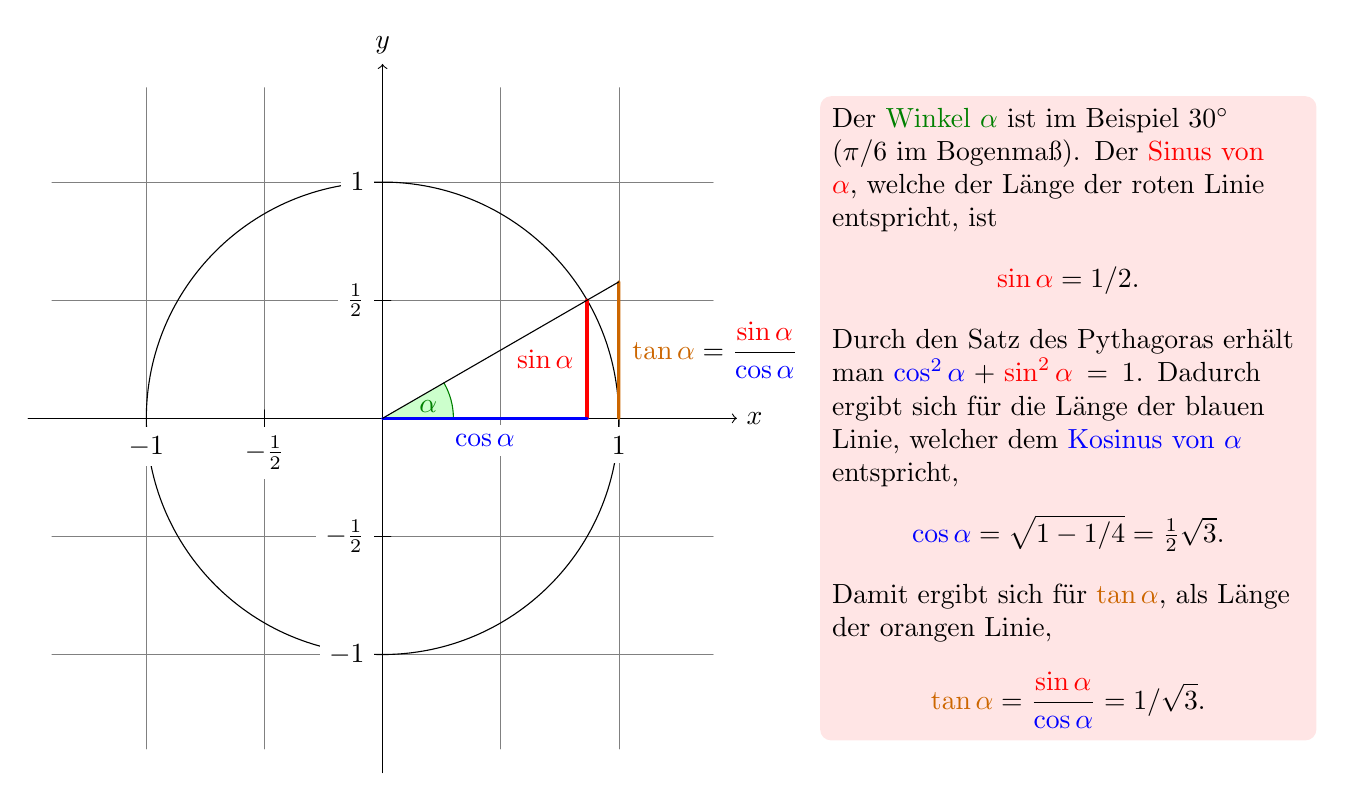
\begin{tikzpicture}[scale=3,cap=round]
  % Local definitions
  \def\costhirty{0.8660256}

  % Colors
  \colorlet{anglecolor}{green!50!black}
  \colorlet{sincolor}{red}
  \colorlet{tancolor}{orange!80!black}
  \colorlet{coscolor}{blue}

  % Styles
  \tikzstyle{axes}=[]
  \tikzstyle{important line}=[very thick]
  \tikzstyle{information text}=[rounded corners,fill=red!10,inner sep=1ex]

  % The graphic
  \draw[style=help lines,step=0.5cm] (-1.4,-1.4) grid (1.4,1.4);

  \draw (0,0) circle (1cm);

  \begin{scope}[style=axes]
    \draw[->] (-1.5,0) -- (1.5,0) node[right] {$x$};
    \draw[->] (0,-1.5) -- (0,1.5) node[above] {$y$};

    \foreach \x/\xtext in {-1, -.5/-\frac{1}{2}, 1}
      \draw[xshift=\x cm] (0pt,1pt) -- (0pt,-1pt) node[below,fill=white]
            {$\xtext$};

    \foreach \y/\ytext in {-1, -.5/-\frac{1}{2}, .5/\frac{1}{2}, 1}
      \draw[yshift=\y cm] (1pt,0pt) -- (-1pt,0pt) node[left,fill=white]
            {$\ytext$};
  \end{scope}

  \filldraw[fill=green!20,draw=anglecolor] (0,0) -- (3mm,0pt) arc(0:30:3mm);
  \draw (15:2mm) node[anglecolor] {$\alpha$};

  \draw[style=important line,sincolor]
    (30:1cm) -- node[left=1pt,fill=white] {$\sin \alpha$} +(0,-.5);

  \draw[style=important line,coscolor]
    (0,0) -- node[below=2pt,fill=white] {$\cos \alpha$} (\costhirty,0);

  \draw[style=important line,tancolor] (1,0) --
    node [right=1pt,fill=white]
    {
      $\displaystyle \tan \alpha \color{black}=
      \frac{{\color{sincolor}\sin \alpha}}{\color{coscolor}\cos \alpha}$
    } (intersection of 0,0--30:1cm and 1,0--1,1) coordinate (t);

  \draw (0,0) -- (t);

  \draw[xshift=1.85cm] node [right,text width=6cm,style=information text]
    {
      Der {\color{anglecolor} Winkel $\alpha$} ist im Beispiel $30^\circ$  ($\pi/6$ im Bogenmaß). Der {\color{sincolor}Sinus von
        $\alpha$}, welche der Länge der roten Linie entspricht, ist
      \[
      {\color{sincolor} \sin \alpha} = 1/2.
      \]
      Durch den Satz des Pythagoras erhält man ${\color{coscolor}\cos^2 \alpha} +
      {\color{sincolor}\sin^2\alpha} =1$. Dadurch ergibt sich für die Länge der blauen Linie, welcher dem {\color{coscolor}Kosinus von $\alpha$} entspricht, 
      \[
      {\color{coscolor}\cos\alpha} = \sqrt{1 - 1/4} = \textstyle
      \frac{1}{2} \sqrt 3.
      \]%
     Damit ergibt sich für {\color{tancolor}$\tan \alpha$}, als Länge der orangen Linie,
      \[
      {\color{tancolor}\tan\alpha} = \frac{{\color{sincolor}\sin
          \alpha}}{\color{coscolor}\cos \alpha} = 1/\sqrt 3.
      \]%
    };
\end{tikzpicture}
\end{center}
\subsection{Sinus und Kosinus als Funktionen}
Erfolgt der Übergang vom Gradmaß (Winkel in $^{\circ}$) in das Bogenmaß (entsprechnende Länge des Kreisbogens) ist es möglich eine Funktion mit reellen Definitionsbereich zu definieren.
Beim Übergang von Sinus und Kosinus auf das Bogenmaß und beliebige Winkel ergibt sich die entsprechende Funktion.
\begin{b8d}{Die Sinus- und Kosinusfunktion}{}
 Die Funktion $f$ mit  $f(x) = \sin{(x)}$ mit $\mathds{D}_f = \mathds{R}$ und $\mathds{W}_f = [-1;1]$ nennt man Sinusfunktion.\\
 Die Funktion $g$ mit  $g(x) = \cos{(x)}$ mit $\mathds{D}_g = \mathds{R}$ und $\mathds{W}_g = [-1;1]$ nennt man Kosinusfunktion. 

\begin{center}
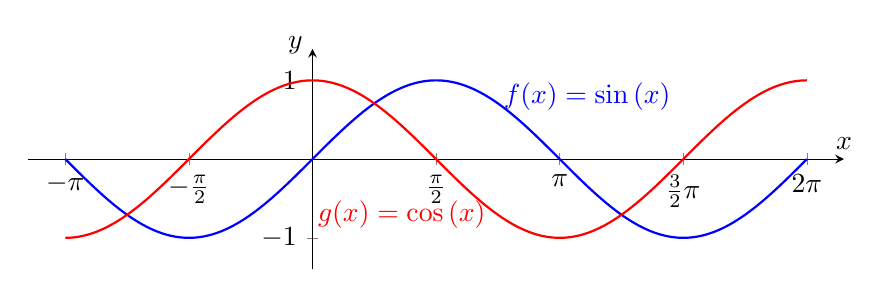
\begin{tikzpicture}
  \begin{axis}[
      axis lines = middle, 
      xlabel=$x$, 
      xlabel style={at=(current axis.right of origin), anchor=south},
      ylabel=$y$, 
      ylabel style={at=(current axis.above origin), anchor=base east},
      xmin=-180,xmax=360,ymin=-1,ymax=1,
      xtick = {-180,-90,...,360},
      xticklabels = {$-\pi$,$-\frac{\pi}{2}$,0,$\frac{\pi}{2}$,$\pi$,$\frac{3}{2}\pi$,$2\pi$},
      ytick ={-1,0,1},
      yticklabels ={$-1$,$0$,$1$},
      enlarge x limits=.05,
      enlarge y limits=.2,
      y=1cm,% <- ergänzt
      x=0.017444cm% <- ergänzt
      ]

\addplot[blue,thick,samples=300,domain=-180:360]{sin(x)};
\addplot[red,thick,samples=300,domain=-180:360]{cos(x)};

\draw[blue] (200,0.5)   node [above] {$f(x)= \sin{(x)}$};
\draw[red] (65,-1)   node [above] {$g(x)= \cos{(x)}$};
\end{axis}
\end{tikzpicture} 
\end{center}
Die Sinuskurve und die Kosinuskurve verlaufen periodisch, das heißt, dass sich ein einzelner Abschnitt wieder und wieder wiederholt. Man kann auch sagen, dass sich die Funktionswerte ($y$) im selben Abstand wiederholen. Die kleinste Periode der Kurven entspricht einer Wellenbewegung oberhalb und unterhalb der x-Achse. In der oberen Abbildung erkennt man, dass die kleinste Periode über die Länge von $2\pi$ geht.
\end{b8d}
\label{GraphSinCos}
\begin{merke}{Eigenschaften der Sinus- und Kosinuskurve}{} \phantomsection\label{SinCosEigenschaften}
    Durch die Periodizität der Kurven ergeben sich für besondere Punkte Regelmäßigkeiten.
    \begin{enumerate}
        \item Sinusfunktion
    \begin{itemize}
        \item Die Nullstellen der Sinuskurve liegen bei allen ganzzahligen Vielfachen von $\pi$. $$x_{0} = k\cdot \pi \hspace{0.5cm} \text{mit} \hspace{0.5cm} k\in \mathds{N}$$
        \item Die relativen Maxima liegen bei $$x_{Max} = \dfrac{\pi}{2} + 2\cdot k\cdot \pi \hspace{0.5cm} \text{mit} \hspace{0.5cm} k\in \mathds{N}$$
        \item Die relativen Minima liegen bei $$x_{Min} = \dfrac{3}{2}\cdot \pi + 2\cdot k\cdot \pi \hspace{0.5cm} \text{mit} \hspace{0.5cm} k\in \mathds{N}$$
    \end{itemize}
    \item Kosinuskurve
    \begin{itemize}
        \item Die Nullstellen der Kosinuskurve liegen bei allen ganzzahligen Vielfachen von $\dfrac{\pi}{2}$. $$x_{0} = \dfrac{\pi}{2}+ k \cdot \pi\hspace{0.5cm} \text{mit} \hspace{0.5cm} k\in \mathds{N}$$
        \item Die relativen Maxima liegen bei $$x_{Max} = k\cdot 2\cdot\pi \hspace{0.5cm} \text{mit} \hspace{0.5cm} k\in \mathds{N}$$
        \item Die relativen Minima liegen bei $$x_{Min} =  \pi + 2\cdot k\cdot \pi \hspace{0.5cm} \text{mit} \hspace{0.5cm} k\in \mathds{N}$$
    \end{itemize}
        \end{enumerate}
Wie man anhand dieser Zusammenstellung leicht sehen kann, ist die Kosinuskurve eine um $\dfrac{\pi}{2}$ verschobene Sinuskurve.
\end{merke}
\subsection{Die allgemeine Sinusfunktion}
\begin{b8d}{Die allgemeine Sinusfunktion}{}\index{Funktionen!Trigonometrische!allgemeiner Sinus} \label{SinCosAllgFunkt}
    Die allgemeine Sinusfunktion lautet $$f(x)= a\cdot \sin{(b\cdot (x - c))}+d \hspace{0.25cm} \text{mit} \hspace{0.25cm} a\in \mathds{R}\setminus\{0\} \hspace{0.25cm} \text{und} \hspace{0.25cm} b,c,d \in \mathds{R}$$
    Die vier Parameter verändern die Sinuskurve wie folgt:
    \begin{itemize}
        \item Der Parameter a ändert die Amplitute, also die maximale Auslenkung der Kurve
        \item Der Parameter b streckt bzw. staucht die Kurve in Richtung der x-Achse. Durch den Faktor b wird damit die Periode $p$ verändert $p = \dfrac{2\cdot \pi}{b}$
        \item Der Parameter c verschiebt die Kurve in Richtung der x-Achse.
        \item Der Parameter d verschiebt die Kurve in Richtung der x-Achse.
    \end{itemize}
\end{b8d}
\begin{center}
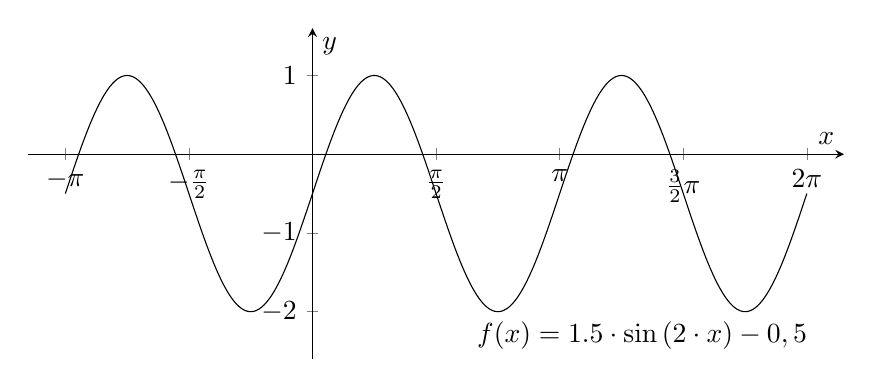
\begin{tikzpicture}
  \begin{axis}[
      axis lines = middle, 
      xlabel=$x$, 
      ylabel=$y$, 
      xmin=-180,xmax=360,ymin=-2,ymax=1,
      xtick = {-180,-90,...,360},     
      xticklabels = {$-\pi$,$-\frac{\pi}{2}$,0,$\frac{\pi}{2}$,$\pi$,$\frac{3}{2}\pi$,$2\pi$},
      ytick ={-2,-1,0,1},
      yticklabels ={$-2$,$-1$,$0$,$1$},
      enlarge x limits=.05,
      enlarge y limits=.2,
      y=1cm,% <- ergänzt
      x=0.017444cm,% <- ergänzt
      ]
\addplot[samples=300,domain=-180:360]{1.5*sin(2*x)-0.5};
%\addplot[red,thick,samples=300,domain=-180:360]{cos(x)};

\draw (240,-2.6)   node [above] {$f(x)= 1.5\cdot \sin{(2\cdot x) -0,5}$};
\end{axis}
\end{tikzpicture} 
\end{center}
\section{Potenz- und Logarithmengesetze}
Um mit den $e$- und  $\ln$-Funktionen arbeiten zu können müssen die Potenz- und Logarithmengesetze beherrscht werden.
\subsection{Potenzgesetze}
Um mit Potenzen zu rechnen gibt es einige wichtige Gesetzmäßigkeiten.
\begin{merke}{Die Potenzgesetze}{} \index{Potenzgesetze}
\begin{itemize}
    \item $a^0 = 1$ für alle $a\in \mathds{R}\setminus\{0\}$
    \item $a^1 =a$ für alle $a\in \mathds{R}\setminus\{0\}$
    \item $a^{-n} = \dfrac{1}{a^n}$ für alle $a>0$ und $n \in \mathds{R}$
    \item $a^n \cdot a^m = a^{n+m}$ für alle $a>0$ und $n,m \in \mathds{R}$
    \item $a^n : a^m = \dfrac{a^n}{a^m} = a^{n-m}$ für alle $a>0$ und $n,m \in \mathds{R}$
    \item $(a\cdot b)^n = a^n \cdot b^n$ für alle $a,b>0$ und $n,m \in \mathds{R}$
    \item $\left(\dfrac{a}{b}\right)^n = \dfrac{a^n}{b^n}$ für alle $a,b>0$ und $n,m \in \mathds{R}$
    \item $ \left( a^n \right)^m = a^{n\cdot m}$ für alle $a>0$ und $n,m \in \mathds{R}$
    \item $a^{\frac{n}{m}} = \sqrt[m]{a^m} = \left( \sqrt[n]{a}\right)^m$ für alle $a>0$ und $n,m \in \mathds{N}$
\end{itemize}
\end{merke}
\subsection{Logarithmengesetze}\index{Logarithmus}
In der Mathematik bezeichnte der Logarithmus den Exponenten mit dem die Basis potenziert werden muss um eine bestimmte Zahl zu erhalten. Es gilt damit also folgender Zusammenhang $$a^n = b \Leftrightarrow n = \log_a (b)$$
Der Logarithmus ist nur für Zahlen $a,b>0$ mit $a,b\in\mathds{R}$ definiert. Um Logarithmen vereinfachen zu können gelten einige grundlegende Regeln. 
\begin{merke}{Logarithmenregeln}{}\index{Logarithmus!Rechenregeln}
Für folgende Umformungen gilt $a,b,x,y > 0$ für die Basen $a,b$ gilt zusätzlich $a,b \neq 1$.
\begin{itemize}
    \item Produktregel: $\log_a{(x\cdot y)} = \log_a{(x)} + \log_a{(y)}$
    \item Quotientenregel: $\log_a{\left(\dfrac{x}{y}\right)}= \log_a{(x)} -\log_a{(y)}$
    \item Exponetenregel: $\log_a{(x^r)} = r\cdot \log_a{(x)}$ mit $r\in \mathds{R}$
    \item Kettenregel: $\log_a{\left(\dfrac{1}{x}\right)} = -1\cdot\log_a{(x)}$
    \item Basisumrechnung: $\log_a{(x)} = \dfrac{\log_b{(x)}}{\log_b{(a)}}$
\end{itemize}
\end{merke}
Zur Vereinfachung werden bei speziellen Logarithmen Abkürzungen in der Schreibweise verwendet.
\begin{bem}{Abkürzungen}{}\index{Logarithmus!Abkürzungen}\phantomsection\label{ln}
    \begin{itemize}
        \item $\log_{10}{(n)} = \lg{(n)}$ 
        \item $\log_{2}{(n)} = \text{ld}{(n)}$
        \item $\log_{e}{(n)} = \ln{(n)}$
    \end{itemize}
\end{bem}
\subsection{Exponentialgleichungen}\index{Logarithmus!Exponentialgleichungen}
In der Mathematik ist es häufig notwendig, dass man Exponentialgleichungen löst. Diese Gleichungen lassen sich auf 3 Fälle zurückführen. 
\begin{enumerate}
    \item $c\cdot a^n = b $ 
    \item $c\cdot a^n = b\cdot d^m$
    \item $a^n=a^m$
\end{enumerate}
Anhand von Beispiele sollen die drei Fälle besprochen werden.
\begin{bsp}{Exponentialgleichung 1}{}
Gegeben ist die Gleichung $6\cdot 1,4^x = 9$.
\begin{equation*}
    \begin{split}
        6\cdot 1,4^x &= 9 \hspace{0.5cm} | : 6\\
        1,4^x&= \dfrac{3}{2} \hspace{0.5cm} | \log_{1,4}{()}\\
        x&= \log_{1,4}{(\frac{3}{2})} \approx 1,21
    \end{split}
\end{equation*}
\end{bsp}
\begin{bsp}{Exponentialgleichung 2}{}
Gegeben ist die Gleichung $2\cdot 1,2^{2x} = 5\cdot 2^{-x}$.
\begin{equation*}
    \begin{split}
        2\cdot 1,2^{2x} &= 5\cdot 2^{-x} \hspace{0.5cm} | \ln{()}\\
        \ln{(2\cdot 1,2^{2x})} &= \ln{(5\cdot 2^{-x})} \hspace{0.5cm}| \text{ Anwendung der Logarithmengesetze}\\
        \ln{(2)} + \ln{(1,2^{2x})} &= \ln{(5)} + \ln{(2^{-x})}\\
        \ln{(2)} + 2x\cdot \ln{(1,2)} &= \ln{(5)} +(-x) \cdot \ln{(2)} \hspace{0.5cm} | + x \cdot \ln{(2)}; -\ln{(2)}\\
          2x\cdot \ln{(1,2)} + x \cdot \ln{(2)} &= \ln{(5)} -\ln{(2)}\\
          x\cdot \left(2\cdot \ln{(1,2)} + \ln{(2)} \right) &= \ln{(\frac{5}{2})}\\
          x\cdot \ln{(1,2^2 \cdot 2)}&= \ln{(\frac{5}{2})}\\
           x\cdot \ln{(2,88)}&= \ln{(\frac{5}{2})}\hspace{0.5cm}| :\ln{(2,88)}\\
           x&= \dfrac{\ln{(\frac{5}{2})}}{\ln{(2,88)}} \approx 0.87
    \end{split}
\end{equation*}
\end{bsp}
\begin{bsp}{Exponentialgleichung 3}{}
Gegeben ist die Gleichung $2^{3x} =2^{\frac{1}{2}x-3}$.
\begin{equation*}
    \begin{split}
    2^{3x} &=2^{\frac{1}{2}x-3} \hspace{0.5cm}| \text{ Gleichung ist durch Exponentenvergleich lösbar}\\
    3x&= \frac{1}{2}x-3  \hspace{0.5cm}| - \frac{1}{2}x\\
    2,5x &=-3 \hspace{0.5cm}|:2,5\\
    x&= -\dfrac{6}{5}
    \end{split}
\end{equation*}
\end{bsp}
Bei einigen Gleichungen lohnt sich die Substitution zum lösen. hierbei wird die Gleichung auf eine Gleichung zurückgeführt, die einfacher zu lösen ist.
\begin{bsp}{Substitution bei Logarithmen}{}\index{Logarithmus!Substitution}
Gegeben ist die Gleichung $5^{2x} -2\cdot 5^x -8 =0$. Diese Gleichung kann vereinfacht werden, indem man $5^x$ mit dem Parameter $u$ substituiert.
\begin{equation*}
    \begin{split}
     5^{2x} -2\cdot 5^x -8 &=0\\
     5^x\cdot 5^x -2\cdot 5^x -8 &=0\hspace{0.5cm} | \text{ Substitution von } 5^x=u\\
        u^2 -2\cdot u -8 &=0\\
        u_{1/2} &= \dfrac{2\pm \sqrt{(-2)^2 -4\cdot 1\cdot (-8)}}{2\cdot 1}\\
        &=\dfrac{2\pm \sqrt{4+32}}{2}\\
        &=\dfrac{2\pm \sqrt{36}}{2}\\
        &= \dfrac{2\pm 6}{2}\\
        u_1 &= 4\\
        u_2 &= -2 
    \end{split}
\end{equation*}
Durch die Substitution wurden die beiden rechnerischen Lösungen $u_1$ und $u_2$ gefunden. Diese Müssen jetzt rücksubstituiert werden. Für $u_1$ ergibt sich damit folgendes
\begin{equation*}
    \begin{split}
u_1&=4\\
5^x&=4\hspace{0.5cm} | \ln{()}\\
\ln{(5^x)}&= \ln{(4)}\\
x\cdot\ln{(5)} &= \ln{(4)}\hspace{0.5cm }| : \ln{(5)}\\
x&= \dfrac{\ln{(4)} }{\ln{(5)} } \approx 0,86
    \end{split}
\end{equation*}
Für den Wert $u_2 = -2$ kann keine Lösung gefunden werden, da $5^x > 0$ für alle Werte von $x$ ist. Damit ist $5^x= -2$ nicht lösbar.\\
Aus diesen Rechnungen folgt damit, dass nur $x=\dfrac{\ln{(4)} }{\ln{(5)} } $ die Gleichung $5^{2x} -2\cdot 5^x -8 =0$ löst.
\end{bsp}